%%%%%%%%%%%%%%%%%%%%%%%%%%%%%%%%%%%%%%%%%%%%%%%%%%%%%%%%%%%%%%%%%%%%%%%%%%%%%%%%%%%%%
% PACOTES                                                                           %
%%%%%%%%%%%%%%%%%%%%%%%%%%%%%%%%%%%%%%%%%%%%%%%%%%%%%%%%%%%%%%%%%%%%%%%%%%%%%%%%%%%%%
\documentclass[a4paper,12pt]{article}

%-----------------------------------------------------------------------------------%
% LAYOUT DA PÁGINA                                                                  %
%-----------------------------------------------------------------------------------%
\usepackage[top=2.75cm, bottom=2.75cm, left=2.75cm, right=2.75cm]{geometry}
%\usepackage{fancyhdr} % Permite controlar como são exibidos os cabeçalhos

%-----------------------------------------------------------------------------------%
% FORMATAÇÃO DO TEXTO                                                               %
%-----------------------------------------------------------------------------------%
%\usepackage{setspace} % Permite definir o espaçamento entre linhas

%-----------------------------------------------------------------------------------%
% PACOTES DE IMAGENS                                                                %
%-----------------------------------------------------------------------------------%
\usepackage[pdftex]{graphicx}
\pdfsuppresswarningpagegroup=1 % A warning issued when several PDF images are
% imported in the same page. Mostly harmless, can be almost always supressed.
%\usepackage[pstarrows]{pict2e} % Amplia as funcionalidades do ambiente picture
\usepackage{tikz}
\usetikzlibrary{shapes, arrows, arrows.meta}

%-----------------------------------------------------------------------------------%
% PACOTES DE TABELAS                                                                %
%-----------------------------------------------------------------------------------%
\usepackage{array} % Facilita a formatação de tabelas
%\usepackage{multirow} % Permite criar células que ocupam várias linhas em uma tabela
\usepackage{longtable} % Permite criar tabelas que quebram de página

%-----------------------------------------------------------------------------------%
% PACOTES MATEMÁTICOS DE BASE                                                       %
%-----------------------------------------------------------------------------------%
\usepackage{amsfonts,amstext,amscd,bezier,amsthm,amssymb}
\usepackage[centertags]{amsmath}

%-----------------------------------------------------------------------------------%
% PACOTES DE SÍMBOLOS MATEMÁTICOS                                                   %
%-----------------------------------------------------------------------------------%
\usepackage{mathtools} % Símbolos matemáticos extras. (ex.: \xrightharpoon)
%\usepackage[integrals]{wasysym} % Muda o estilo das integrais, além de outros
%                                 símbolos extras
%\usepackage[nice]{nicefrac} % Permite o uso de frações "melhores". Usar \nicefrac{}{}

%-----------------------------------------------------------------------------------%
% PACOTES DE FONTES MATEMÁTICAS                                                     %
%-----------------------------------------------------------------------------------%
%\usepackage{mathbbol} % Quase todos os símbolos com \mathbb
%\usepackage{bbm} % Extensão dos símbolos de \mathbb. Usar comando \mathbbm
%\usepackage{calrsfs} % Muda o estilo de \mathcal
%\usepackage[mathcal]{euscript} % Muda o estilo de \mathcal

%-----------------------------------------------------------------------------------%
% PACOTES DE CODIFICAÇÃO DE FONTES                                                  %
%-----------------------------------------------------------------------------------%
\usepackage[utf8]{inputenc} % Permite o uso de caracteres ISO 8859-1, incluindo os
%                               caracteres acentuados diretamente.
\usepackage[T1]{fontenc} % Uso de fontes T1, necessário para tratar caracteres
%                          acentuados como um único bloco.

%-----------------------------------------------------------------------------------%
% PACOTES DE LÍNGUAS                                                                %
%-----------------------------------------------------------------------------------%
\usepackage[french]{babel} % Seleciona a língua do documento, definindo nomes de
%                              seções, nome do índice, da bibliografia, etc. Em caso
%                              de documento com mais de uma língua, a padrão é a
%                              última.
\NoAutoSpaceBeforeFDP % Utilizar em francês se quiser evitar espaços antes de :

%-----------------------------------------------------------------------------------%
% PACOTES DE BIBLIOGRAFIA                                                           %
%-----------------------------------------------------------------------------------%
%\usepackage{babelbib} % Permite definir a língua das entradas da bibliografia. Usar
%                       [fixlanguage] para uma mesma língua para todas as entradas e
%                       \selectbiblanguage{} para definir a língua. Um estilo compa-
%                       tível com babelbib deve ser usado (ex: babplain)
\usepackage{cite} % Organiza os elementos citados dentro de um mesmo \cite.

%-----------------------------------------------------------------------------------%
% PACOTES DE FONTES                                                                 %
%-----------------------------------------------------------------------------------%
% Computer Modern (fonte padrão)                                                    %
% - - - - - - - - - - - - - - - - - - - - - - - - - - - - - - - - - - - - - - - - - %
%\usepackage{ae} % A usar com a fonte padrão do LaTeX quando forem gerados PDFs, para
%                 corrigir erros de visualização

% Computer Modern Bright (sans serif)                                               %
% - - - - - - - - - - - - - - - - - - - - - - - - - - - - - - - - - - - - - - - - - %
%\usepackage{cmbright}

% Times New Roman                                                                   %
% - - - - - - - - - - - - - - - - - - - - - - - - - - - - - - - - - - - - - - - - - %
%\usepackage{mathptmx} % Muda texto e modo matemático
%\usepackage{times} % Apenas texto, não muda modo matemático

% Arial                                                                             %
% - - - - - - - - - - - - - - - - - - - - - - - - - - - - - - - - - - - - - - - - - %
%\usepackage[scaled]{uarial} % Arial como fonte sans serif padrão

% Palatino                                                                          %
% - - - - - - - - - - - - - - - - - - - - - - - - - - - - - - - - - - - - - - - - - %
%\usepackage{mathpazo} % Muda texto e modo matemático
%\usepackage{palatino} % Apenas texto, não muda modo matemático

% Concrete                                                                          %
% - - - - - - - - - - - - - - - - - - - - - - - - - - - - - - - - - - - - - - - - - %
%\usepackage{ccfonts} % Texto: Concrete; Matemático: Concrete Math
%\usepackage{ccfonts, eulervm} % Texto: Concrete; Matemático: Euler

% Iwona                                                                             %
% - - - - - - - - - - - - - - - - - - - - - - - - - - - - - - - - - - - - - - - - - %
%\usepackage[math]{iwona} % Texto e modo matemático: Iwona

% Kurier                                                                            %
% - - - - - - - - - - - - - - - - - - - - - - - - - - - - - - - - - - - - - - - - - %
%\usepackage[math]{kurier} % Texto e modo matemático: Kurier

% Antykwa Póltawskiego                                                              %
% - - - - - - - - - - - - - - - - - - - - - - - - - - - - - - - - - - - - - - - - - %
%\usepackage{antpolt} % Texto: Antykwa Póltawskiego; Matemático: nenhum
                     % Usar fontenc = QX ou OT4

% Utopia                                                                            %
% - - - - - - - - - - - - - - - - - - - - - - - - - - - - - - - - - - - - - - - - - %                     
%\usepackage{fourier} % Texto: Utopia; Matemático: Fourier

% KP Serif                                                                          %
% - - - - - - - - - - - - - - - - - - - - - - - - - - - - - - - - - - - - - - - - - %
\usepackage{kpfonts}

%-----------------------------------------------------------------------------------%
% CORES                                                                             %
%-----------------------------------------------------------------------------------%
\usepackage{color}
\definecolor{darkgreen}{rgb}{0,0.5,0}
\definecolor{darkmagenta}{rgb}{0.5,0,0.5}
\definecolor{darkgray}{rgb}{0.5,0.5,0.5}
\definecolor{darkblue}{rgb}{0.2,0.2,0.4}
\definecolor{darkred}{rgb}{0.6,0.15,0.15}
\definecolor{gray}{rgb}{0.65,0.65,0.65}
\definecolor{lightgray}{rgb}{0.8,0.8,0.8}
\definecolor{lightblue}{rgb}{0.5,0.5,1}
\definecolor{lightgreen}{rgb}{0.5,1,0.5}
\definecolor{deadred}{rgb}{0.7, 0.2, 0.2}
\definecolor{deadblue}{rgb}{0.2, 0.2, 0.7}

%-----------------------------------------------------------------------------------%
% PACOTES DIVERSOS                                                                  %
%-----------------------------------------------------------------------------------%
\usepackage{icomma} % Permite uso de vírgula como separador decimal
\usepackage{url} % Pacote para não ter problemas com URLs. Usar \url{}
%\usepackage{randtext} % Troca a ordem de letras de uma frase (útil com e-mails em
                      % PDFs a serem publicados on-line.
\usepackage[hidelinks]{hyperref}
%\usepackage{showkeys} % Para mostrar o nome dos labels
\usepackage{enumitem} % Facilita o uso de listas, inclusive referências a itens de
                      % listas.
%\usepackage[absolute]{textpos} % Posição absoluta de texto na página
%\usepackage{pdfpages} % Permite incluir documentos em PDF no arquivo
%\usepackage{refcheck} % Verifica as referências procurando por
%                      % labels não usados ou equações numeradas sem labels.
%                      % Verificar o arquivo .log e procurar por RefCheck.
\usepackage[french, onelanguage]{algorithm2e}

%%%%%%%%%%%%%%%%%%%%%%%%%%%%%%%%%%%%%%%%%%%%%%%%%%%%%%%%%%%%%%%%%%%%%%%%%%%%%%%%%%%%%
% CONFIGURAÇÕES                                                                     %
%%%%%%%%%%%%%%%%%%%%%%%%%%%%%%%%%%%%%%%%%%%%%%%%%%%%%%%%%%%%%%%%%%%%%%%%%%%%%%%%%%%%%

%-----------------------------------------------------------------------------------%
% FORMATAÇÃO DO TEXTO                                                               %
%-----------------------------------------------------------------------------------%
%\onehalfspacing % Espaçamento 1 1/2 (definido no pacote setspace)

%-----------------------------------------------------------------------------------%
% DEFINIÇÃO DE AMBIENTES MATEMÁTICOS                                                %
%-----------------------------------------------------------------------------------%
%\theoremstyle{plain}
%\newtheorem{theo}{Teorema}[section]
%\newtheorem{lemm}[theo]{Lema}
%\newtheorem{coro}[theo]{Corolário}
%\newtheorem{prop}[theo]{Proposição}
%\theoremstyle{definition}
%\newtheorem{defi}[theo]{Definição}
%\newtheorem{remq}[theo]{Observação}
%%\newtheorem{expl}[theo]{Exemplo}
%\newenvironment{expl}%
%  {\refstepcounter{theo}%
%    \begin{list}{}{%
%    \setlength{\topsep}{0pt}%
%    \setlength{\leftmargin}{\parindent}%
%    \setlength{\rightmargin}{0pt}%
%    \setlength{\listparindent}{\parindent}%
%    \setlength{\itemindent}{0pt}%
%    \setlength{\parsep}{\parskip}}%
%    \item[]{\bf Exemplo \thetheo. }}%
%  {\hspace*{\fill} $\square$ \end{list} \medskip}
%\newenvironment{solu}%
%  {\noindent {\bf Solução. }\small}%
%  {\hspace*{\fill} $\square$ \normalsize \medskip}
%\newenvironment{dems}[1][Demonstração]%
%  {\begin{list}{}{%
%    \setlength{\topsep}{0pt}%
%    \setlength{\leftmargin}{\parindent}%
%    \setlength{\rightmargin}{0pt}%
%    \setlength{\listparindent}{\parindent}%
%    \setlength{\itemindent}{0pt}%
%    \setlength{\parsep}{\parskip}}%
%    \item[]{\bf #1. }}%
%  {\hspace*{\fill} $\blacksquare$ \end{list} \medskip}


%-----------------------------------------------------------------------------------%
% DEFINIÇÃO DE COMANDOS MATEMÁTICOS                                                 %
%-----------------------------------------------------------------------------------%
%\newcommand*\diff{\mathop{}\!\mathrm{d}}

%\newcommand{\norm}[1]{\left\lVert #1\right\lVert} % Norma
%\newcommand{\abs}[1]{\left\lvert #1\right \rvert} % Valor absoluto
%\newcommand{\floor}[1]{\left\lfloor #1 \right\rfloor} % Arredondar para baixo
%\newcommand{\ceil}[1]{\left\lceil #1 \right\rceil} % Arredondar para cima
\DeclarePairedDelimiter{\ceil}{\lceil}{\rceil}
\DeclareMathOperator*{\argmax}{argmax}

%-----------------------------------------------------------------------------------%
% NUMERAÇÃO DE ELEMENTOS                                                            %
%-----------------------------------------------------------------------------------%
%\numberwithin{table}{section}
%\numberwithin{table}{subsection}
%\numberwithin{figure}{section}
%\numberwithin{figure}{subsection}
%\numberwithin{equation}{section}
%\numberwithin{equation}{subsection}
%\numberwithin{theo}{chapter}
%\numberwithin{theo}{subsection}

% Maximal percentage of the page occupied by floats
\renewcommand\floatpagefraction{.9}
\renewcommand\topfraction{.9}
\renewcommand\bottomfraction{.9}
\renewcommand\textfraction{.1}
% Maximal number of floats per page
\setcounter{totalnumber}{50}
\setcounter{topnumber}{50}
\setcounter{bottomnumber}{50}

%%%%%%%%%%%%%%%%%%%%%%%%%%%%%%%%%%%%%%%%%%%%%%%%%%%%%%%%%%%%%%%%%%%%%%%%%%%%%%%%%%%%%
% ESTRUTURA DO DOCUMENTO                                                            %
%%%%%%%%%%%%%%%%%%%%%%%%%%%%%%%%%%%%%%%%%%%%%%%%%%%%%%%%%%%%%%%%%%%%%%%%%%%%%%%%%%%%%
\begin{document}

\pagestyle{plain}

\title{3I008 --- Projet \\ ORush \\ Partie 2 : Interface graphique}
\author{Ariana Carnielli}
\date{}

\maketitle

\sloppy

\tableofcontents

\section{Introduction}

Dans cette deuxième partie du projet, après l'implémentation du noyau du jeu \emph{ORush} avec des fonctions permettant la manipulation des états, l'implémentation des mouvements et la résolution automatique d'une grille, cette deuxième partie du projet s'intéresse à l'implémentation d'une interface graphique pour le jeu. Pour cela, on a utilisé l'interopérabilité entre OCaml et JavaScript à l'aide de l'API \verb@gen_js_api@, qui se base sur le compilateur \verb@js_of_ocaml@. L'interface du jeu codé est donné dans la Figure \ref{FigORush}. La suite de ce document décrit les techniques utilisées et les principaux choix d'implémentation faits.

\begin{figure}[ht]
\centering
\begin{tabular}{cc}
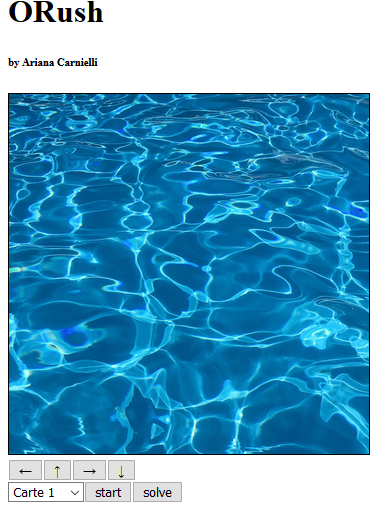
\includegraphics[width=0.45\textwidth]{Figures/ORushStart_} & 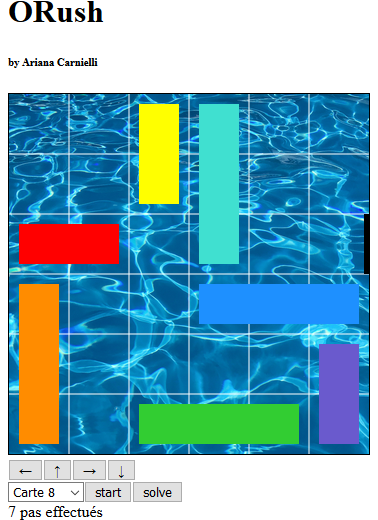
\includegraphics[width=0.45\textwidth]{Figures/ORush_} \tabularnewline
(a) & (b) \tabularnewline
\end{tabular}
\caption{Interface du jeu \emph{ORush} (a) à l'initialisation et (b) au cours de la résolution d'une grille.}
\label{FigORush}
\end{figure}

\section{Fichier HTML}

Le jeu est chargé à travers un fichier \verb@index.html@. Ce fichier est minimaliste : il crée une balise \verb@h1@ pour le titre, un \verb@canvas@ pour le jeu en soi et charge le script principal contenant le jeu à travers une balise \verb@script@. Tous les autres éléments nécessaires pour le jeu, comme les éléments sur le \emph{canvas}, les boutons et le titre de la page sont crées à partir du code OCaml.

\section{Fichiers de la partie 1}

Les fichiers \verb@port.ml@, \verb@moves.ml@ et \verb@solver.ml@ codés à la partie 1 de ce projet sont utilisés dans cette partie et constituent le noyau du jeu. Les versions utilisées sont essentiellement identiques à celles de la partie 1, l'unique différence étant la création de deux fonctions dans \verb@port.ml@ pour permettre d'extraire plus facilement des informations sur un bateau.

\section{Maps}

Un fichier \verb@maps.ml@ a été crée, contenant 14 cartes différentes pour le jeu \emph{ORush} et la palette de couleurs utilisées pour dessiner les bateaux. Il s'agit des 12 cartes fournies en exemple pour la partie 1 plus deux autres crées pour tester d'autres configurations de jeu.

Ce fichier a été crée car il n'a pas été possible de charger automatiquement les cartes depuis des fichiers \verb@.txt@. En effet, la lecture des fichiers à l'aide de la fonction OCaml \verb@open_in@ levait toujours une exception indiquant que le fichier n'avait pas été trouvé. Après des tests en utilisant les fonctions \verb@Sys.getcwd@ et \verb@Sys.readdir@, on a remarqué que le code JavaScript obtenu à partir de la compilation d'OCaml travaillait sur un dossier virtuel \verb@/static/@ qui était vide. La lecture en utilisant le chemin relatif du fichier de tests n'était donc pas possible, et comme la lecture par chemin absolu rendrait le jeu inutilisable sur toute autre machine, on a décidé d'implémenter les cartes comme code en OCaml, permettant donc leur utilisation partout. Cela a cependant l'inconvénient de rendre plus difficile la création de nouvelles cartes.

\section{ORush\_js}

Le fichier \verb@orush_js@ contient la partie principale du code de l'interface graphique. Il contient une fonction \verb@main@, appelée au démarrage du jeu, qui fait les configurations principales, fixant la taille du \emph{canvas} à 360px $\times$ 360px, affichant le titre du jeu et les boutons de contrôle et déclarant toutes les \emph{listeners} associés aux boutons, au \emph{canvas} et aux flèches du clavier. Cette fonction principale contient aussi des variables mutables contenant l'état courant du jeu, le numéro de la carte courante, le bateau sélectionné, un compteur de mouvement et la solution donnée par le solveur automatique. Ces variables sont modifiées par les fonctions \emph{listeners} quand nécessaire, le choix de les implémenter comme mutables provient du fait que les fonctions \emph{listeners} doivent obligatoirement retourner un \verb@unit@.

\subsection{Début d'une partie}

Le jeu commence lorsque l'utilisateur appuie sur le bouton \verb@start@, qui appelle la fonction homonyme. Cette fonction nettoie l'écran à l'aide d'une fonction dédiée \verb@clear_canvas@, dessine les lignes horizontales et verticales constituant le grid et la sortie à l'aide de la fonction \verb@set_grid@, cherche l'état sélectionné dans le menu et redémarre toutes les variables mutables créées dans \verb@main@. Elle garantit aussi que les flèches sont habilitées et que le bouton permettant de faire un nouveau pas de la solution automatique n'est pas affiché.

La fonction \verb@start@ se charge aussi d'afficher l'état initial du jeu. L'affichage d'un état du jeu est fait par la fonction \verb@draw_state@, qui ne fait que parcourir la liste de bateaux d'un état et les afficher par la fonction \verb@draw_boat@. Cette fonction dessine chaque bateau comme un rectangle, à une distance de 10px des bords de la case, avec des couleurs différentes basées sur la lettre qui représente le bateau.

\subsection{Solution automatique}

L'utilisateur a toujours l'option de demander la solution du jeu, à travers le bouton \verb@solve@. Ce bouton appelle la fonction \verb@solve_start@, qui calcule la solution automatique à partir de l'état courant, fait apparaitre un nouveau bouton \verb@next step@, affiche la solution dans une balise \verb@div@ créée au préalable pour ce but et désactive les touches du clavier, les boutons de flèche et le bouton \verb@solve@ lui-même. Chaque clic dans \verb@next step@ appelle la fonction \verb@solve_step@, qui met l'écran à jour avec le prochain pas de la solution, incrémente le compteur de mouvements et, à la fin, réactive les boutons qui étaient déactives et cache le bouton \verb@next step@. Si l'utilisateur appuie sur \verb@start@ avant la fin de la solution, le jeu redémarre et les boutons sont réactivés. Si l'utilisateur a choisi de rester sur la même grille, l'affichage de la solution reste à l'écran ; sinon, il est effacé.

\subsection{Sélection d'un bateau}

La sélection d'un bateau se fait par un clic de la souris sur le bateau correspondant (ou sur l'espace entre le bateau et le bord de sa case). Par défaut, le bateau A est sélectionné lorsqu'une grille est chargée. La sélection d'un bateau lors d'un clic se fait par un \emph{listener} de clics sur le \emph{canvas}, qui appelle la fonction \verb@boat_of_click@. Cette fonction calcule la case correspondante à partir des coordonnées du clic relatives au coin en haut à gauche du \emph{canvas} et utilise la fonction \verb@Port.grid_of_state@ pour déterminer quel bateau a été sélectionné. Un clic dans une case ne contenant pas de bateau désélectionne tout bateau (ce qui correspond à affecter le caractère \verb@'~'@ à la variable de \verb@main@ contenant le bateau courant).

\subsection{Mouvement d'un bateau}

Le mouvement d'un bateau peut être fait par les boutons de flèches de l'interface ou par les flèches du clavier. Pour ce faire, outre les \emph{listeners} de chaque bouton, un \emph{listener} a aussi été codé pour le clavier en attendant l'évènement \verb@keydown@. Lors de cet évènement, si la touche appuyée est une des flèches du clavier (codes 37 à 40) et on n'est pas dans le mode de solution automatique, on appelle la fonction \verb@move_of_click@, qui est aussi appelée par les boutons.

La fonction \verb@move_of_click@ vérifie d'abord qu'un bateau est bien sélectionné avant de faire tout mouvement. Elle crée ensuite un mouvement et essaie de l'appliquer à l'aide de la fonction \verb@Moves.apply_move@, en ignorant tout mouvement à gauche ou à droite des bateaux dans la verticale ou vers le haut ou le bas des bateaux à l'horizontale. Si le mouvement peut être appliqué, cette fonction se charge aussi de le faire et de mettre à jour l'état courant et le dessin à l'écran. Si l'utilisateur gagne la partie, elle affiche aussi une fenêtre avec un message contenant le nombre de pas réalisés. Si le mouvement n'est pas possible, la fonction l'ignore.

\section{Makefile}

Pour compiler le jeu, un fichier \verb@Makefile@ a été crée basé sur celui donné dans le TME11. On a rajouté la compilation des fichiers de la partie 1 du projet ainsi que du nouveau fichier \verb@maps.ml@ et adapté la compilation par \verb@js_of_ocaml@ de notre fichier principal \verb@ocaml_js.ml@.

Ce fichier \verb@Makefile@ doit connaitre l'emplacement du dossier \verb@opam@ et des fichiers de la version \verb@4.06.1@ d'OCaml. Ce dossier est typiquement \verb@~/.opam/4.06.1@, cependant l'utilisation de ce chemin donne une erreur de compilation avec \verb@js_of_ocaml@. En effet, \verb@js_of_ocaml@ semble incapable de trouver le fichier \verb@findlib.conf@ dans \verb@~/.opam/4.06.1/lib/@, mais il le trouve sans problèmes si \verb@~@ est remplacé par le chemin absolu du répertoire personnel. Ainsi, une variable \verb@OPAM_PATH@ est rajoutée au début du \verb@Makefile@ et doit être modifiée avant la compilation pour contenir le chemin absolu vers la version \verb@4.06.1@ dans \verb@.opam@.

\end{document}
